\documentclass[working]{tuftebook}

\usepackage[utf8]{inputenc}
\usepackage[T1]{fontenc}
\usepackage{textcomp}

\usepackage{url}

\usepackage[
    sorting=nyt,
    style=alphabetic
]{biblatex}
\addbibresource{bibliography.bib}

\usepackage{hyperref}
\hypersetup{
    colorlinks,
    linkcolor={black},
    citecolor={black},
    urlcolor={blue!80!black}
}
\usepackage[noabbrev]{cleveref}

% Adds Bibliography, ... to Table of Contents
\usepackage[nottoc]{tocbibind}

\usepackage{graphicx}
\usepackage{float}
\usepackage[usenames,dvipsnames,svgnames]{xcolor}

% \usepackage{cmbright}

\usepackage{amsmath, amsfonts, mathtools, amsthm, amssymb}
\usepackage{mathrsfs}
\usepackage{cancel}

\usepackage{tikz}
\usepackage{tikz-cd}

% theorems
\usepackage{thmtools}
\usepackage{thm-restate}
\usepackage[framemethod=TikZ]{mdframed}
\mdfsetup{skipabove=1em,skipbelow=0em, innertopmargin=12pt, innerbottommargin=8pt}

\theoremstyle{definition}

\makeatletter

\declaretheoremstyle[headfont=\bfseries\sffamily, bodyfont=\normalfont, mdframed={ nobreak } ]{thmgreenbox}
\declaretheoremstyle[headfont=\bfseries\sffamily, bodyfont=\normalfont, mdframed={ nobreak } ]{thmredbox}
\declaretheoremstyle[headfont=\bfseries\sffamily, bodyfont=\normalfont]{thmbluebox}
\declaretheoremstyle[headfont=\bfseries\sffamily, bodyfont=\normalfont]{thmblueline}
\declaretheoremstyle[headfont=\bfseries\sffamily, bodyfont=\normalfont, numbered=no, mdframed={ rightline=false, topline=false, bottomline=false, }, qed=\qedsymbol ]{thmproofbox}
\declaretheoremstyle[headfont=\bfseries\sffamily, bodyfont=\normalfont, numbered=no, mdframed={ nobreak, rightline=false, topline=false, bottomline=false } ]{thmexplanationbox}

\declaretheoremstyle[headfont=\bfseries\sffamily, bodyfont=\normalfont, numbered=no, mdframed={ nobreak, rightline=false, topline=false, bottomline=false } ]{thmexplanationbox}


\declaretheorem[numberwithin=chapter, style=thmgreenbox, name=Definition]{definition}
\declaretheorem[sibling=definition, style=thmredbox, name=Corollary]{corollary}
\declaretheorem[sibling=definition, style=thmredbox, name=Proposition]{prop}
\declaretheorem[sibling=definition, style=thmredbox, name=Theorem]{theorem}
\declaretheorem[sibling=definition, style=thmredbox, name=Lemma]{lemma}
\declaretheorem[sibling=definition, style=thmbluebox,  name=Example]{eg}
\declaretheorem[sibling=definition, style=thmbluebox,  name=Nonexample]{noneg}
\declaretheorem[sibling=definition, style=thmblueline, name=Remark]{remark}
\declaretheorem[sibling=definition, style=thmredbox, name=Axiom]{axiom}




\declaretheorem[numbered=no, style=thmexplanationbox, name=Proof]{explanation}
\declaretheorem[numbered=no, style=thmproofbox, name=Proof]{replacementproof}
\declaretheorem[style=thmbluebox,  numbered=no, name=Exercise]{ex}
\declaretheorem[style=thmblueline, numbered=no, name=Note]{note}

% \renewenvironment{proof}[1][\proofname]{\begin{replacementproof}}{\end{replacementproof}}

% \AtEndEnvironment{eg}{\null\hfill$\diamond$}%

\newtheorem*{uovt}{UOVT}
\newtheorem*{notation}{Notation}
\newtheorem*{previouslyseen}{As previously seen}
\newtheorem*{problem}{Problem}
\newtheorem*{observe}{Observe}
\newtheorem*{property}{Property}
\newtheorem*{intuition}{Intuition}


\declaretheoremstyle[
    headfont=\bfseries\sffamily\color{RawSienna!70!black}, bodyfont=\normalfont,
    mdframed={
        linewidth=2pt,
        rightline=false, topline=false, bottomline=false,
        linecolor=RawSienna, backgroundcolor=RawSienna!5,
    }
]{todo}
\declaretheorem[numbered=no, style=todo, name=TODO]{TODO}


\usepackage{etoolbox}
\AtEndEnvironment{vb}{\null\hfill$\diamond$}%
\AtEndEnvironment{intermezzo}{\null\hfill$\diamond$}%

% http://tex.stackexchange.com/questions/22119/how-can-i-change-the-spacing-before-theorems-with-amsthm
% \def\thm@space@setup{%
%   \thm@preskip=\parskip \thm@postskip=0pt
% }

\usepackage{xifthen}

\makeatother

% figure support (https://castel.dev/post/lecture-notes-2)
\usepackage{import}
\usepackage{xifthen}
\pdfminorversion=7
\usepackage{pdfpages}
\usepackage{transparent}


\makeatletter
\newif\ifworking
\@ifclasswith{tuftebook}{working}{\workingtrue}{\workingfalse}
\makeatother

\newcommand{\incfig}[2][1]{%
    % \ifworking{\makebox[0pt][c]{\color{gray}{\scriptsize\textsf{#2}}}}\fi%
    \def\svgwidth{#1\textwidth}
    \import{./figures/}{#2.pdf_tex}
}

\newcommand{\fullwidthincfig}[2][0.90]{%
    % \ifworking{\makebox[0pt][l]{\color{gray}{\scriptsize\textsf{#2}}}}\fi%
    \def\svgwidth{#1\paperwidth}
    \import{./figures/}{#2.pdf_tex}
}



\newcommand{\minifig}[2]{%
    \def\svgwidth{#1}%
    \begingroup%
    \setbox0=\hbox{\import{./figures/}{#2.pdf_tex}}%
    \parbox{\wd0}{\box0}\endgroup%
    \hspace*{0.2cm}
}

% %http://tex.stackexchange.com/questions/76273/multiple-pdfs-with-page-group-included-in-a-single-page-warning
\pdfsuppresswarningpagegroup=1

\newcommand\todo[1]{\ifworking {{\color{red}{#1}}} \else {}\fi}
\newcommand\charlotte[1]{\ifworking {{\color{blue}{#1}}} \else {}\fi}

\author{Rasmus Curt Raschke}



\usepackage{multirow}
\def\block(#1,#2)#3{\multicolumn{#2}{c}{\multirow{#1}{*}{$ #3 $}}}

% \overfullrule=1mm

\newenvironment{myproof}[1][\proofname]{%
  \proof[\rm \bf #1]%
}{\endproof}


\let\oldphi\phi
\let\phi\varphi
\let\varphi\oldphi

% Algebra
\DeclareMathOperator{\Hom}{\text{Hom}}
\DeclareMathOperator{\ord}{\text{ord}}
\DeclareMathOperator{\Ann}{\text{Ann}}
\DeclareMathOperator{\Gal}{\text{Gal}}
\DeclareMathOperator{\Aut}{\text{Aut}}

% Analysis

% Category

% Differential Geometry
\DeclareMathOperator{\Ric}{Ric}
\DeclareMathOperator{\ric}{ric}
\newcommand{\inj}{\text{inj}}
\DeclareMathOperator{\gst}{g_{st}}
\newcommand{\hodge}{{\star}}

% Topology


\usepackage{enumitem}
\newlist{abbrv}{itemize}{1}
\setlist[abbrv,1]{label=,labelwidth=1in,align=parleft,itemsep=0.1\baselineskip,leftmargin=!}

\DeclareMathOperator{\Crit}{Crit}
\newcommand{\Cinfty}{C^\infty}

\newcommand{\stable}[1]{W^s(#1)}
\newcommand{\unstable}[1]{W^u(#1)}
\newcommand{\unstableb}[1]{\overline{W}^u(#1)}

\def\symbolentry#1#2#3{\item[#2] #3}
\def\sort#1{}

\makeatletter
\newcommand{\superimpose}[2]{%
  {\ooalign{$#1\@firstoftwo#2$\cr\hfil$#1\@secondoftwo#2$\hfil\cr}}}
\makeatother

% https://tex.stackexchange.com/questions/134863/command-for-transverse-and-not-pitchfork-as-used-in-guillemin-and-pollack
% \newcommand{\tcap}{\mathrel{\mathpalette\superimpose{{\raise0.15ex\hbox{$\top$}}{\cap}}}}
\newcommand{\tcap}{\pitchfork}

\newcommand\traj[2]{\mathcal M(#1, #2)}
\renewcommand\L[2]{\mathcal L(#1, #2)}
\newcommand\Lb[2]{\overline{\mathcal L}(#1, #2)}

\newcommand\nX[3]{n_{#1}(#2, #3)}
\newcommand\NX[3]{N_{#1}(#2, #3)}
\newcommand\HM[3][]{HM_{#1}(C_\bul(#2), \partial_#3)}
\newcommand\HMf[2][]{HM_{#1}(#2)}

\DeclareMathOperator{\Ind}{Ind}
\DeclareMathOperator{\Rank}{Rank}

\DeclareMathOperator{\codim}{codim}
\DeclareMathOperator{\grad}{grad}

\DeclareMathOperator{\Ker}{Ker}
\renewcommand{\Im}{\operatorname{Im}}

\newcommand\sphere[1]{S^{#1}}
\newcommand\cdisk[1]{B^{#1}}
\newcommand\odisk[1]{D^{#1}}
\newcommand\bul{\bullet}

 % \newcommand{\bigstar}{\mathop{\Huge \mathlarger{\mathlarger{*}}}}



\newcommand{\listofsymbols}{
    \chapter*{List of symbols}
    \begin{abbrv}


        % \symbolentry{U}{$U(\epsilon, \eta)$}{Morse chart}
        \symbolentry{0}{$M \tcap N$}{Transverse intersection}
    \end{abbrv}
}

\newcommand{\tpoinc}[1]{\ensuremath{\mathrm P_{\text{top}}^{#1}}}
\newcommand{\spoinc}[1]{\ensuremath{\mathrm P_{\infty}^{#1}}}
\newcommand{\ppoinc}[1]{\ensuremath{\mathrm P_{\text{PL}}^{#1}}}
\newcommand{\cpoinc}[1]{\ensuremath{\mathrm P_{C}^{#1}}}

\newcommand{\tcob}[1]{\ensuremath{\mathrm H_{\text{top}}^{#1}}}
\newcommand{\scob}[1]{\ensuremath{\mathrm H_{\infty}^{#1}}}
\newcommand{\pcob}[1]{\ensuremath{\mathrm H_{\text{PL}}^{#1}}}
\newcommand{\ccob}[1]{\ensuremath{\mathrm H_{C}^{#1}}}

\newcommand{\mant}{\ensuremath{\textsf{Man}_{\text{top}}}}
\newcommand{\mans}{\ensuremath{\textsf{Man}_{\infty}}}
\newcommand{\manp}{\ensuremath{\textsf{Man}_{\text{PL}}}}

\usepackage{booktabs}
\usepackage{array}
\newcommand{\overview}[7]{
    \smallskip
    \begin{center}
        \begin{tabular}{
                >{\centering\arraybackslash}p{1.3cm}%
                >{\centering\arraybackslash}p{1.3cm}%
                >{\centering\arraybackslash}p{1.3cm}%
                >{}p{0.3cm}%
                >{\centering\arraybackslash}p{1.3cm}%
                >{\centering\arraybackslash}p{1.3cm}%
                >{\centering\arraybackslash}p{1.3cm}}
                \tpoinc{#1} & \ppoinc{#1} & \spoinc{#1} && \tcob{#1} & \pcob{#1} & \scob{#1}\\
                #2   & #3 & #4 & & #5 & #6 & #7
        \end{tabular}
    \end{center}
}

\usepackage{pdfpages}

\usepackage{lipsum}
\usepackage{parskip}
\usepackage{titletoc}

\newcommand\circled[1]{
    \begin{tikzpicture}[baseline=(char.base)]%
        \node[circle,draw,inner sep=1pt] (char) {\textsf{#1}};%
\end{tikzpicture}}
% minicircle for in figures!
\newcommand\mc[1]{\footnotesize\circled{#1}}

\usepackage{cmbright}
\usepackage{bm}

% \usepackage{eso-pic}                % put things into background 
% \usepackage{lipsum}                 % for sample text

% \definecolor{reallylightgray}{HTML}{FAFAFA}
% \AddToShipoutPicture{% from package eso-pic: put something to the background
%     \ifthenelse{\isodd{\thepage}}{
%           % ODD page: left bar
%           \AtPageLowerLeft{% start the bar at the left bottom of the page
%             \put(\LenToUnit{\dimexpr\paperwidth-222pt},0){% move it to the top right
%                 \color{reallylightgray}\rule{222pt}{297mm}%
%               }%
%           }%
%       }%
%       {%
%         \AtPageLowerLeft{% put it at the left bottom of the page
%           \color{reallylightgray}\rule{222pt}{297mm}%
%         }%
%    }%
% }

\title{Classical Magnetic Systems}
\date{Academic year 2025--2026}
\begin{document}
    
    \renewcommand{\thepage}{\roman{page}}
    \thispagestyle{empty}
    \pagestyle{plain}
    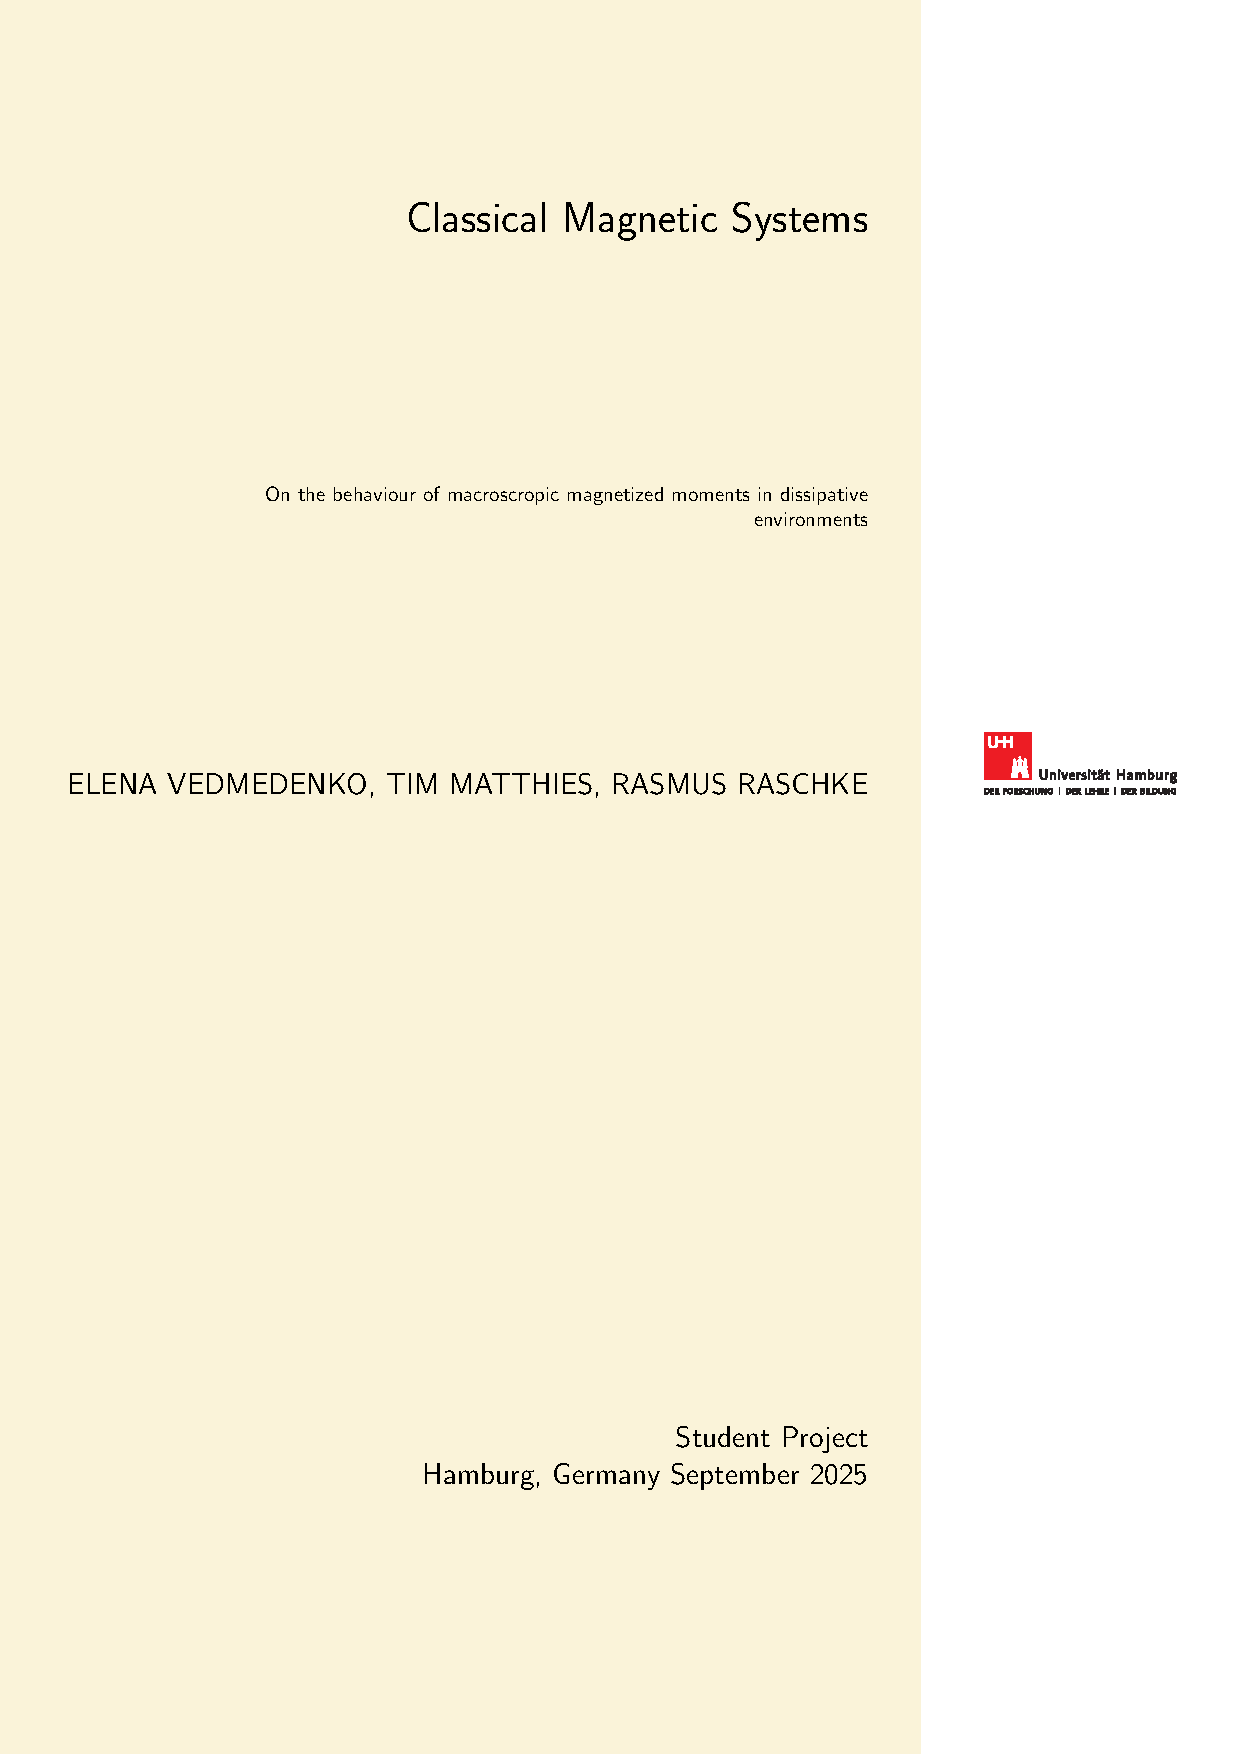
\includepdf{frontpage/front.pdf}
    \setcounter{page}{0}
    \chapter*{Preface}
\label{ch:preface}
\addcontentsline{toc}{chapter}{\nameref{ch:preface}}

This document contains my work in regard to the magnetospin effect, first discribed by Dr. Elena Vedmedenko, who proprosed this topic to me, and Tim Matthies, who already conducted fundational investigations. My goal is to derive an accurate mathematical description of this effect, leading to accurate computational simulations of the discribed systems.

\hfill \emph{Raschke, August 2025}

    \listofsymbols
    \tableofcontents
    \cleardoublepage
    \renewcommand{\thepage}{\arabic{page}}
    \setcounter{page}{1}
    \pagestyle{normal}
    \chapter{Mathematical Introduction}
\label{chap:matint}
\vspace*{-0.9cm}

% \startcontents[chapters]
% \printcontents[chapters]{}{1}{}

We start with the necessary mathematical theory. If the reader already feels comfortable with the theory of smooth manifolds, variational calculus on aforementioned spaces, (Lie) groups as well as autonomous differential equations, they may skip this chapter. We assume basic knowledge of linear algebra and calculus.

\section{Group Theory}
We need some fundamental group theory. From here on, all vector spaces are finite-dimensional.
\begin{definition}[Group]
\marginnote{One should think of groups in terms of symmetries: A symmetry of an abstract object can be thought of as a collection of operations leaving said object invariant.}
A \textbf{Group} is a pair $(G, \circ)$ consisting of a set $G$ and an operation $\circ$ such that the following axioms are satisfied:
\begin{itemize}
    \item $\forall a,b,c \in G: a \circ (b \circ c) = (a \circ b) \circ c$
    \item $\forall a \in G \, \exists a^{-1} \in G: a \circ a^{-1} = 1$
    \item $\exists e \in G \, \forall a \in G: e \circ a = a$
\end{itemize}
If the operation is commutative, we call the group \textbf{abelian}.
\end{definition}
There are plenty of examples of groups important in physics:
\begin{eg}
\marginnote{
        Note that every vector space over $\mathbb{R}$ has a basis. Choosing one and representing automorphisms as $n \times n$-matrices yields the usual group structure by matrix multiplication. This also clearly demonstrates that groups of linear maps cannot be abelian in general.}
    Let $V$ be a real vector space. The automorphisms $V \to V$ consitute a group under composition, the \emph{general linear group} of dimension $n$, $\GL_n(V)$.
    There are several important subgroups of $\GL(\mathbb{R}^n)$ we will heavily use later. Let \[\langle \cdot, \cdot \rangle: \mathbb{R}^n \to \mathbb{R}\] be the euclidean scalar product on $\mathbb{R}^n$ and $T \in \GL(\mathbb{R}^n)$. We define the \emph{orthogonal group} as
\[\O(n):=\{Q \in \GL(\mathbb{R}^n) \mid QQ^top = Q^\top Q = \id\} \leq \GL(\mathbb{R}^n).\]  
Further restricting our attention to orthogonal automorphisms with unit determinant yields the \emph{special orthogonal group} \[
    \SO(n) := \{R \in \O(n) \mid \det R = 1\} \leq \O(n).
.\] 
\end{eg}
In physics, we are usually concerned with how a certain group acts on a physical system. For that, we need actions and representations.
\begin{definition}[Group Action]
    Let $G$ be a group with identity $e$ and $M$ be a set. A \textbf{right-action} of $G$ on $M$ is a map \[
    \alpha: G \times X \to X
    .\] 
    such that:
    \begin{itemize}
        \item $\alpha(e,x) = x$
        \item $\alpha(h, \alpha(g,x))=\alpha(gh,x)$
    \end{itemize}
    is satisfied. We write $G \acts M$ and $\alpha(g,x)=:g.x$ for short.
\end{definition}
\begin{definition}[Representation]
    Let $V$ be a real vector space and $G$ be a group. A \textbf{real $G$-representation} is a group homomorphism \[
    \rho: V \to \GL(V)
    .\] 
    We call $V$ \textbf{representation space} and $\deg V$ the degree of the representation.
    
\end{definition}
\section{Configuration Manifolds and Lie groups}

\begin{definition}[Topological Manifold]
    A \textbf{topological $n$-manifold} is a topological space $M$ such that:
    \begin{itemize}
        \item $M$ has the Hausdorff property.
        \item $M$ is second-countable.
        \item $M$ is locally euclidean: For every $p \in M$ there is an open neighbourhood $U \subseteq M$ of $p$ and a homeomorphism $\phi: U \to V$ such that $V \subseteq \mathbb{R}^n$ is open. We call $(\phi, U)$ a \textbf{chart} on $M$.
    \end{itemize}
\end{definition}
Since we want to apply the formalism in concrete examples, we will often work in local coordinates. Note that with the standard basis of $\mathbb{R}^n$, we can write a chart map as 
\[
\phi(p)=(\phi_1(p), \dots, \phi_n(p)) =: (x^1(p), \dots, x^n(p))
.\] where $x^i: M \to \mathbb{R}$ are the chart components. Since the charts are homeomorphisms, they can be locally inverted to a map $\phi^{-1}: V \to U$, in which case we call $\phi^{-1}$ a \emph{local parametrization} of $M$.
\begin{eg}
    \begin{itemize}
        \item Trivially, the real euclidean space $\mathbb{R}^n$ is an $n$-dimensional smooth manifold with the identity $\id$ being a global chart.
        \item The $n$-sphere $\mathbb{S}^n$ is a smooth manifold with local charts given by projection onto the coordinate axes.
    \item The $n$-torus \[T^n = \underbrace{\mathbb{S} \times \cdots \times \mathbb{S}}_{n\text{ times}}\] is a smooth $n$-manifold. In the case of $T^2$, one obtains local charts easily as the $2$-torus is a surface of revolution. 
    \end{itemize}
\end{eg}
We need the notion of smoothness on manifolds.
\begin{definition}[Smooth Manifold]
    \marginnote{Note that with this, we get a notion of smooth maps on abstract manifolds: If $M,N$ are smooth manifolds and $F: M \to N$ is a map, we call it smooth if for every $p \in M$ there is a chart $(U,\phi)$ with $p \in U$ and a smooth chart $(V, \psi)$ with $F(p) \in V$ such that \[ \psi \circ F \circ \phi^{-1}: \mathbb{R}^m \to \mathbb{R}^n\] is smooth in the usual sense.}
    A \textbf{maximal atlas} for a topological manifold $M$ is a collection $\mathfrak{A}$ of charts of $M$ such that every $p \in M$ is contained in some chart and $\mathfrak{A}$ is not properly contained in some other atlas. We call $\mathfrak{A}$ smooth if for any two charts $(U,\phi),(V,\psi) \in \mathfrak{A}$ we have either $U \cap V = \emptyset$ or \[
        \phi^{-1} \circ \psi: V \to U
    .\] is a smooth ($\mathcal{C}^\infty$) map, called \textbf{chart transition map}. A \textbf{smooth manifold} is a pair $(M, \mathfrak{A})$ such that $M$ is a topological manifold and $\mathfrak{A}$ is a maximal smooth atlas.
\end{definition}
There are many examples important to physics:
\begin{eg}
    \begin{itemize}
        \item The $\mathbb{R}^n$ obtains a smooth maximal atlas by means of the identity.
        \item The sphere $\mathbb{S}^2$ has a smooth atlas with two charts $\mathbb{S}^2 \setminus N$ and $\mathbb{S}^2 \setminus S$, where $N$ and $S$ are north and south pole, respectively. The chart map is given by the \emph{stereographic projection} $\sigma: \mathbb{S}^2 \setminus N \to \mathbb{R}^2$. 
        \item Any finite-dimensional real normed vector space $V$ is a smooth manifold. The choice of a basis determines an isomorphism $\mathbb{R}^n \cong V$ which we take as global chart. For any other basis, one obtains a basis transformation matrix which is linear, hence a $\mathcal{C}^\infty$ chart transition.
        \item Any open subset $U \subseteq \mathbb{R}^n$ is a smooth manifold on its own with the smooth atlas $\{U, \id_U\}$. We call such a manifold an \emph{open submanifold} of $\mathbb{R}^n$.
    \end{itemize}
\end{eg}
\section{Variational Calculus}

\section{Ordinary Differential Equations}

    \chapter{Magnetic Ball on an Incline}
\label{chap:incline}
\vspace*{-0.9cm}

% \startcontents[chapters]
% \printcontents[chapters]{}{1}{}

\section{Two-Dimensional System}
\label{sec:twodim}
\subsection*{Lagrangian Equation of Motion}
We start our investigation by considering a very simplified model of a rigid two-dimensional disk of mass $M$ with a constant magnetic moment $\mathbf{m}$ rolling on an inclined plane of length $l$ and angle $\alpha$ without slipping in the earth magnetic field $\mathbf{B}$. The moment of inertia is $I=\frac{MR^2}{2}$. Similar to the example of semi-holonomic constraints, our generalized coordinates are the rolling distance $q$ and the rotational angle $\theta$. Note that while $\mathbf{m}$ is constant in the rolling frame of the disk, the angle between $\mathbf{m}$ and $\mathbf{B}$ changes with the rolling motion. We have again the same semi-holonomic constraint 
\[
dq-Rd\theta = 0
.\] This is a first integral, yielding \[
q(t) - q_0= R\theta(t) - \theta_0 
\] where we set $q_0:=q(0)$ and $\theta_0 := \theta(0)$. For simplicity, we choose the coordinates in such a way that w.l.o.g. $q_0=0=\theta_0$. The kinetic energy is given by
\[
    T(q, \dot{q}) = \frac{M}{2} \|\dot{q}\|^2 + \frac{I}{2} \|\dot{\theta}\|^2 = \frac{3M}{4} \dot{q}^2
\] where we substituted $\theta = \frac{q}{R}$. We have two potentials acting on the disk, the first being gravity
\[
    U_\text{g}(q) = Mgh = (q-l)Mg \sin \alpha
.\] The second is due to the magnetic moment of the disk interacting with the earth field. Assuming an ideal magnetic dipole interaction, the potential is governed by the angle between $\mathbf{m}$ and $\mathbf{B}$. 
\marginnote{Allowing $\beta$ to be arbitrary is probably not necessary for the practical experiment as the dipole will align itself with the outer field if one does not impair this movement until the disk starts rolling.}
Assuming an initial angle of $\beta$ at $t=0$, the angle at time $t$ is simply $\beta + \theta$. Therefore, the electromagnetic potential is
\[
    U_\text{em}(q)=- \langle \mathbf{m}, \mathbf{B} \rangle = -mB\cos(\beta + \frac{x}{R})
\] with $m=\|\mathbf{m}\|$ and $B=\|\mathbf{B}\|^2$.\\
We obtain the Lagrangian
\[
    \mathcal{L}(q,\dot{q})= T-U_\text{g}-U_\text{em}= \frac{3M}{4} \|\dot{q}(t)\|^2+ (l-q(t))Mg\sin \alpha + mB \cos\left(\beta + \frac{q(t)}{R}\right)
\] which gives rise to just one Lagrangian equation of the second kind:
\begin{equation}
    \frac{d}{dt} \left( \frac{\partial \mathcal{L}}{\partial \dot{q}}\right) - \frac{\partial \mathcal{L}}{\partial q}= 0
\end{equation}
This yields the ODE \[
    \ddot{q}(t)= \frac{2g}{3} \sin \alpha  + \frac{2mB}{3MR}\sin\left(\beta + \frac{q}{R}\right) = f(q(t))
\] which is a second-order autonomous ODE. We already discussed how to solve such an equation. The first integral needed is
\begin{align*}
    \int_{q_0=0}^q f(\tau) \, d\tau &= \int_{q_0=0}^q \left( \frac{2g}{3}\sin \alpha + \frac{2mB}{3MR} \sin \left(\beta + \frac{q}{R} \right) \right)\, d\tau \\
                                  &= \frac{2g}{3}\sin(\alpha)q - \frac{2mB}{3M} \left( \cos\left(\beta + \frac{q}{R}\right)- \cos\beta\right)
\end{align*}
We make some abbreviations to keep everything readable. Define $A:= \frac{4g}{3} \sin \alpha$, $B := -\frac{4mB}{3M}$ and $C:=\frac{4mB}{3M} \cos \beta$. The implicit solution is then given by
\begin{equation}
t = \pm \int_0^{q(t)} \frac{1}{\sqrt{Aq - B \cos(\beta + \frac{q}{R}) + C}} \, dq.
\end{equation}
The bad news is that this integral cannot be solved analytically. The only option is to calculate the integral numerically, for example my means of a Taylor series, and then invert pointwise to obtain $q=q(t)$. We will focus on some aspects which can be derived in limiting cases.
\subsection*{Symmetries}
The derived Lagrangian is not very abundant in symmeties. As $\mathcal{L}$ is autonomous, the system admits time translation symmetry and hence conservation of energy. However, this is not very surprising as we did not enforce the rolling condition by means of a dissipative Lagrangian but instead as semi-holonomic integrable constraint. The variable $q$ does appear explicitly in the Lagrangian, so it can not be cyclic. The only symmetry remains time symmetry. 

\subsection*{Conclusion}
While it is quite surprising that such a simple system does not admit a closed-form analytic solution, we gain some first insight in the general usefulness of the Lagrangian formalism to derive equations of motion. However, our hope to solve the more complicated three-dimensional system is very much reduced, expecially since the three-dimensional rolling constraint is not always semi-holonomic.



    \printbibliography

\end{document}
